%% BioMed_Central_Tex_Template_v1.06
%%                                      %
%  bmc_article.tex            ver: 1.06 %
%                                       %

%%IMPORTANT: do not delete the first line of this template
%%It must be present to enable the BMC Submission system to
%%recognise this template!!

%%%%%%%%%%%%%%%%%%%%%%%%%%%%%%%%%%%%%%%%%
%%                                     %%
%%  LaTeX template for BioMed Central  %%
%%     journal article submissions     %%
%%                                     %%
%%          <8 June 2012>              %%
%%                                     %%
%%                                     %%
%%%%%%%%%%%%%%%%%%%%%%%%%%%%%%%%%%%%%%%%%


%%%%%%%%%%%%%%%%%%%%%%%%%%%%%%%%%%%%%%%%%%%%%%%%%%%%%%%%%%%%%%%%%%%%%
%%                                                                 %%
%% For instructions on how to fill out this Tex template           %%
%% document please refer to Readme.html and the instructions for   %%
%% authors page on the biomed central website                      %%
%% http://www.biomedcentral.com/info/authors/                      %%
%%                                                                 %%
%% Please do not use \input{...} to include other tex files.       %%
%% Submit your LaTeX manuscript as one .tex document.              %%
%%                                                                 %%
%% All additional figures and files should be attached             %%
%% separately and not embedded in the \TeX\ document itself.       %%
%%                                                                 %%
%% BioMed Central currently use the MikTex distribution of         %%
%% TeX for Windows) of TeX and LaTeX.  This is available from      %%
%% http://www.miktex.org                                           %%
%%                                                                 %%
%%%%%%%%%%%%%%%%%%%%%%%%%%%%%%%%%%%%%%%%%%%%%%%%%%%%%%%%%%%%%%%%%%%%%

%%% additional documentclass options:
%  [doublespacing]
%  [linenumbers]   - put the line numbers on margins

%%% loading packages, author definitions

\documentclass[twocolumn]{bmcart}
%\documentclass{bmcart}

%%% Load packages
%\usepackage{amsthm,amsmath}
%\RequirePackage{natbib}
%\RequirePackage[authoryear]{natbib}% uncomment this for author-year bibliography
%\RequirePackage{hyperref}
\usepackage[utf8]{inputenc} %unicode support


%%%%%%%%%%%%%%%%%%%%%%%%%%%%%%%%%%%%%%%%%%%%%%%%%
%%                                             %%
%%  If you wish to display your graphics for   %%
%%  your own use using includegraphic or       %%
%%  includegraphics, then comment out the      %%
%%  following two lines of code.               %%
%%  NB: These line *must* be included when     %%
%%  submitting to BMC.                         %%
%%  All figure files must be submitted as      %%
%%  separate graphics through the BMC          %%
%%  submission process, not included in the    %%
%%  submitted article.                         %%
%%                                             %%
%%%%%%%%%%%%%%%%%%%%%%%%%%%%%%%%%%%%%%%%%%%%%%%%%


\def\includegraphic{}
\def\includegraphics{}



%%% Put your definitions there:
\startlocaldefs
\usepackage{booktabs}
\usepackage{url}
\usepackage{listings}
\renewcommand{\lstlistingname}{Listing}
\renewcommand{\familydefault}{\sfdefault}
\lstset{basicstyle=\ttfamily}
\endlocaldefs


\begin{document}

\begin{frontmatter}

\begin{fmbox}
\dochead{Research}

%%%%%%%%%%%%%%%%%%%%%%%%%%%%%%%%%%%%%%%%%%%%%%
%%                                          %%
%% Enter the title of your article here     %%
%%                                          %%
%%%%%%%%%%%%%%%%%%%%%%%%%%%%%%%%%%%%%%%%%%%%%%

\title{Wellmap: A file format for 96-well plates}

%%%%%%%%%%%%%%%%%%%%%%%%%%%%%%%%%%%%%%%%%%%%%%
%%                                          %%
%% Enter the authors here                   %%
%%                                          %%
%% Specify information, if available,       %%
%% in the form:                             %%
%%   <key>={<id1>,<id2>}                    %%
%%   <key>=                                 %%
%% Comment or delete the keys which are     %%
%% not used. Repeat \author command as much %%
%% as required.                             %%
%%                                          %%
%%%%%%%%%%%%%%%%%%%%%%%%%%%%%%%%%%%%%%%%%%%%%%

\author[
   addressref={wyss},                   % id's of addresses, e.g. {aff1,aff2}
   email={kale@thekunderts.net}         % email address
]{\inits{KK}\fnm{Kale} \snm{Kundert}}

%%%%%%%%%%%%%%%%%%%%%%%%%%%%%%%%%%%%%%%%%%%%%%
%%                                          %%
%% Enter the authors' addresses here        %%
%%                                          %%
%% Repeat \address commands as much as      %%
%% required.                                %%
%%                                          %%
%%%%%%%%%%%%%%%%%%%%%%%%%%%%%%%%%%%%%%%%%%%%%%

\address[id=wyss]{%
  \orgname{Wyss Institute for Biologically Inspired Engineering, Harvard University},
  \city{Cambridge, Massachusetts},
  \postcode{02138}
  \cny{USA}
}

%%%%%%%%%%%%%%%%%%%%%%%%%%%%%%%%%%%%%%%%%%%%%%
%%                                          %%
%% Enter short notes here                   %%
%%                                          %%
%% Short notes will be after addresses      %%
%% on first page.                           %%
%%                                          %%
%%%%%%%%%%%%%%%%%%%%%%%%%%%%%%%%%%%%%%%%%%%%%%

\begin{artnotes}
%\note{Sample of title note}     % note to the article
\end{artnotes}

%\end{fmbox}% comment this for two column layout

%%%%%%%%%%%%%%%%%%%%%%%%%%%%%%%%%%%%%%%%%%%%%%
%%                                          %%
%% The Abstract begins here                 %%
%%                                          %%
%% Please refer to the Instructions for     %%
%% authors on http://www.biomedcentral.com  %%
%% and include the section headings         %%
%% accordingly for your article type.       %%
%%                                          %%
%%%%%%%%%%%%%%%%%%%%%%%%%%%%%%%%%%%%%%%%%%%%%%

\begin{abstractbox}

\begin{abstract}

\parttitle{Background}
Microplates are ubiquitous in biological research because they make it easy to
collect data for hundreds of different conditions in a single experiment.
Despite this, there is no standard method to annotate the wealth of data
contained in each plate.

\parttitle{Results}
We introduce a new file format, called wellmap, for describing the layout of
wells on microplates. The format is text-based and emphasizes being easy to
read, write, and share. It is capable of describing any layout for any
experiment. It is also accompanied by a tool for generating clear
visualizations of layout files, and a simple API for parsing layout files in
analysis scripts written in python or R.

\parttitle{Conclusions}
We have used wellmap in our own research to annotate data from a
wide variety of experiments, including qPCR and flow cytometry. Given
the large number of experiments that make use of microplates, it is
our hope that other researchers will find this file format as useful
as we have. For complete instructions on how to install and use wellmap,
visit: \url{https://wellmap.rtfd.io}

\end{abstract}

%%%%%%%%%%%%%%%%%%%%%%%%%%%%%%%%%%%%%%%%%%%%%%
%%                                          %%
%% The keywords begin here                  %%
%%                                          %%
%% Put each keyword in separate \kwd{}.     %%
%%                                          %%
%%%%%%%%%%%%%%%%%%%%%%%%%%%%%%%%%%%%%%%%%%%%%%

\begin{keyword}
\kwd{file format}
\kwd{microplate}
\kwd{24-well plate}
\kwd{96-well plate}
\kwd{384-well plate}
\kwd{python}
\kwd{R}
\kwd{TOML}
\end{keyword}

\end{abstractbox}

\end{fmbox}% uncomment this for two column layout

\end{frontmatter}

%%%%%%%%%%%%%%%%%%%%%%%%%%%%%%%%%%%%%%%%%%%%%%
%%                                          %%
%% The Main Body begins here                %%
%%                                          %%
%% Please refer to the instructions for     %%
%% authors on:                              %%
%% http://www.biomedcentral.com/info/authors%%
%% and include the section headings         %%
%% accordingly for your article type.       %%
%%                                          %%
%% See the Results and Discussion section   %%
%% for details on how to create sub-sections%%
%%                                          %%
%% use \cite{...} to cite references        %%
%%  \cite{koon} and                         %%
%%  \cite{oreg,khar,zvai,xjon,schn,pond}    %%
%%  \nocite{smith,marg,hunn,advi,koha,mouse}%%
%%                                          %%
%%%%%%%%%%%%%%%%%%%%%%%%%%%%%%%%%%%%%%%%%%%%%%

\section*{Background}

24-, 96-, and 384-well plates are ubiquitous in biological research because
they make it easy to collect data for hundreds of different conditions in a
single experiment. Once the data have been collected, though, annotating which
conditions were tested in which wells is more of a challenge than it might
seem. These annotations must be easy to create, because a typical scientist
might perform several microplate experiments every day. They must be easy to
check for mistakes, because mislabeling the data could spoil the entire
experiment. They must be easy to understand, because others might need to
interpret the data without the help of the original scientist. And they must be
easy to incorporate into analysis scripts, because the analysis is the ultimate
purpose of the experiment.

In the absence of a standard way to annotate microplate data, a number of ad
hoc approaches have come into wide use. Unfortunately, none of these ad hoc
approaches satisfy all the criteria listed above.  Perhaps the worst approach
is to describe plate layouts in a paper lab notebook. Such descriptions are
easy to create, but hard to share, hard to keep associated with the data, hard
to check for omissions or ambiguities, and impossible to use directly in
analysis scripts.  Another flawed approach is to hard-code layout information
directly into analysis scripts. These scripts are both hard to write and hard
for others to understand. They also encourage copy-and-pasting to perform
similar analyses on different layouts, which makes it harder to fix bugs or
otherwise improve the scripts. A better approach is to record layouts using
spreadsheet files (e.g. CSV, TSV, XLSX). These files are easy to understand,
and can be stored alongside the data so that they are unlikely to be lost. That
said, spreadsheets are highly redundant because each condition must be
specified separately for each well it applies to. This redundancy makes
spreadsheets both tedious to create and prone to mistakes. It is also not
trivial to parse annotations from a spreadsheet and associate them with raw
data for analysis, although there are tools such as
\texttt{plater}~\cite{hughes2020} or \texttt{plate\_maps}~\cite{jones2014} that
can make this easier.  Finally, some instruments come with proprietary software
that can be used to specify plate layouts for experiments involving that
instrument.  These programs usually make it easy to create and visually check
layouts, but they suffer from a lack of flexibility. Analysis is typically
limited to a handful of options pre-programmed into the software, sharing
layouts may require others to purchase the same software (and sometimes even a
computer with the same operating system), some programs have arbitrary limits
on the number of conditions per well or the number of plates per analysis, and
of course, these programs are not available for all instruments or all
experiments. Overall, there is a need for a better way to annotate microplate
data.

Here we address this need by introducing a file format, called wellmap, that
can be used to describe any layout for any kind of microplate experiment. This
file format is easy to write: The syntax is based on the established TOML
markup language~\cite{preston-werner2020}, and can be learned from just a few
examples. There is minimal redundancy, so even complex layouts can be described
succinctly. The file format is easy to check for mistakes: A program is
provided to create visual maps of wellmap files, where any mistakes will stand
out. The file format is easy to share: It is a text-based format, so no special
software is required to read or write it. Additionally, the syntax is
well-documented and intuitive enough that it can be understood even by those
unfamiliar with it. Finally, the file format is easy to parse: Parsers are
provided for python and R, the two most common languages used for the analysis
of biological data. In both languages, the parsed layout is returned as a
tidy~\cite{wickham2014} data frame. We hope that the wellmap file format will
replace the existing methods for annotating microplate data and thereby make
these experiments easier to annotate and analyze.

\section*{Implementation}

The basic wellmap workflow has two steps. The first is to make files describing
the plate layouts for particular experiments, and the second is to write
analysis scripts that make use of the information in those files. Key aspects
of both steps are highlighted below. For more in-depth and up-to-date
information, refer to the online documentation: \url{https://wellmap.rtfd.io} 

\subsection*{Creating wellmap files}

Wellmap files are organized into groups of wells, such as ``row A'', ``columns
3-5'', ``a 2x2 block with A1 in the top left'', etc.  Each well group can be
associated with any number of experimental parameters, such as ``mutant:
Y37A'', ``concentration: 100 µg/mL'', ``timepoint: 30 min'', etc. For example,
the following snippet specifies that row A contains the Y37A
mutant:

\begin{lstlisting}
[row.A]
mutant = 'Y37A'
\end{lstlisting}

As mentioned above, the wellmap file format is based on
TOML~\cite{preston-werner2020}.  Typically, square brackets are used to
identify groups of wells and equals signs are used to set experimental
parameters. Note however that all of the following are equivalent:

\begin{lstlisting}
[row.A]
mutant = 'Y37A'

[row]
A.mutant = 'Y37A'

row.A.mutant = 'Y37A'
\end{lstlisting}


\subsubsection*{Rows, columns, and blocks}

It's important to describe the various well groups that can be specified,
because they are the key to succinctly specifying plate layouts.
Figure~\ref{fig:well-groups} demonstrates most of these groups. Rows, columns,
and blocks are particularly useful. Note that rows are identified by letters
while columns are identified by numbers. If necessary, rows beyond ``Z'' can be
specified as ``AA'', ``AB'', etc. Blocks are identified by a size and a well.
The size is a width followed by a height (separated by an ``x''), and the well
is the top left corner of the block.

\subsubsection*{Patterns}

Groups of wells are commonly arranged in recurring patterns. It's easy to
imagine a layout where the rows alternate between high and low concentrations
of a drug, for example. The wellmap file format includes a succinct syntax to
express patterns like these. The most basic form of this syntax uses commas to
specify multiple positions for a single row, column, block, or well. Refer to
Table~\ref{tab:pattern-syntax} for some examples. Note that the comma-separated
positions must be quoted, because TOML does not allow unquoted keys to contain
commas.

A more advanced form of this syntax can be used to automatically generate
repeating patterns of well groups. This form of the syntax requires exactly
four comma-separated elements. The first, second, and fourth must be valid
positions, and the third must be an ellipsis. The first and fourth positions
define the start and end of the pattern. The offset between the first and
second positions defines the step size.  For wells and blocks, the step size
may differ in the horizontal and vertical dimensions. It must be possible to
get from the start to the end in steps of the given size. Refer again to Table
~\ref{tab:pattern-syntax} for some examples.

\subsubsection*{Multiple plates}

The wellmap file format has full support for layouts spanning multiple
plates. These are two ways to specify such layouts. The first is to
define ``plate'' groups, which encompass all of the wells on a particular
plate. These groups are unique in that they can contain other groups.
For example, the snippet below specifies that all of the wells on
plate ``day1'' have the Y37A mutant, and the wells on row A of that
plate have a concentration of 100 µg/mL:

\begin{lstlisting}
[plate.day1]
mutant = 'Y37A'
[plate.day1.row.A]
conc_ug_mL = 100
\end{lstlisting}

The second way to combine multiple plates in a single layout is to
use the \texttt{meta.concat} field. This field specifies the paths
to one or more external layout files that will be independently loaded
and concatenated to the current layout. This is often useful for making
a single layout that combines several other layouts. For example,
imagine that we collected three replicates on three different plates.
We might want to make a separate layout file for each replicate, so
that we could analyze them individually. We would then want to make
a fourth file that concatenates the three replicates, so that we could
also analyze the combined results.

As a rule of thumb, use plate groups when it wouldn't make sense to
analyze the plates separately, and use concatenated layouts when it
would.

\subsubsection*{Reusing layouts}

It's common for layouts to be reused, in full or in part, between
experiments. For example, we might want to test the same set of samples
with different concentrations of a drug, or to repeat an experiment
with extra controls, or to perform additional replicates, etc. In
situations such as these, it would be redundant and error-prone to
specify a complete layout for each experiment. Instead, the \texttt{meta.include}
field can be used to set default values for each well from one or
more external layout files. Figure~\ref{fig:bradford}, which is
explained in more detail below, contains a good example of this feature.

\subsubsection*{Interleaved wells}

For some experiments, it is necessary to control for the possibility
of position-dependent effects, such as slight temperature gradients
across the plate, by ``interleaving'' conditions between adjacent
rows or columns. Any position-dependent effects will then be canceled
out when the conditions is question are compared. Despite the added
complexity, these layouts can be easily described using the \texttt{irow}
and \texttt{icol} groups. The ``i'' in these names stands for ``interleaved''.
As demonstrated in Figure~\ref{fig:well-groups}, these groups are
basically rows/columns that alternate up and down/right and left.
These groups also are a good demonstration of the expressive power
of the wellmap format, as interleaved layouts are difficult and/or
tedious to unambiguously describe ad hoc.

\subsubsection*{Extra information}

Wellmap files can contain information beyond just the contents of
each well. In fact, they are meant to contain all of the information
necessary for analysis, because keeping this information in one place
makes the analysis easier to understand and reproduce. For example,
the path(s) to the raw data file(s) can be specified via the \texttt{meta.path}
or \texttt{meta.paths} fields, so that the correct data can be loaded
along with the layout. More generally, any parameters specified in
a wellmap file that are not associated with a well group can be directly
accessed by the analysis script. This can be seen in Figure~\ref{fig:bradford},
where a \texttt{{[}bradford{]}} section is used to specify parameters
specific to the Bradford assay.

\subsection*{Checking for mistakes}

Once a layout file has been written, it is important to double-check
that it does not contain any mistakes. The best way to do this is
to look at a visualization of the layout, such as those in Figure~\ref{fig:well-groups}
and Figure~\ref{fig:bradford}. These visualizations were generated
by a command-line program that is distributed with wellmap. Installing
and using this program is quite simple:

\begin{lstlisting}
$ pip install wellmap
$ wellmap path/to/layout.toml
\end{lstlisting}


\subsection*{Parsing wellmap files}

An important feature of the wellmap file format is that it can be
easily parsed for use in analysis scripts. The API, which is available
for both python and R, consists of a single \texttt{load()} function
that parses a layout file and returns a tidy~\cite{wickham2014}
data frame with a row for each well and a column for each experimental
parameter. This data frame can subsequently be merged with the raw
data to associate each data point with the parameters specified in
the layout file. The \texttt{load()} function can also perform this
merge automatically, if sufficient information about the raw data
is provided.

In many cases, converting an existing analysis script to use wellmap
will take little effort and will make the script both simpler and
more powerful. Little effort because the wellmap API uses standard
data types and follows the ``Unix philosophy'' of doing just one
thing (and doing it well)~\cite{raymond2004}. Simpler because any
code that was previously devoted to specifying layout information
can be replaced with a single command to parse a wellmap file. More
powerful because the script will be able to analyze any layout that
provides the expected experimental parameters, regardless of how the
wells are organized on the plate.

\section*{Discussion}

Any project that uses scripts to analyze microplate data can benefit
from wellmap. The file format itself is not specific to any particular
experiment; it simply describes how wells are organized on plates.
In our own research, we have applied wellmap to layouts from a broad
range of experiments including quantitative polymerase chain reaction
(qPCR), flow cytometry, enzyme-linked immunosorbent assays (ELISA),
Bradford assays, Miller assays, and minimum inhibitory concentration
(MIC) assays. Furthermore, incorporating wellmap into a project is
not an onerous process. There are just two steps, both compatible
with any workflow. First, write a short text file describing the layout
of each experiment. Second, adapt any analysis scripts to load information
from the layout files using a simple API.

There are several noteworthy advantages to using wellmap instead
of an ad hoc approach to record plate layouts. The first is that wellmap
makes it easier to write robust, reusable analysis scripts. Because
all of the layout information is specified externally and parsed into
a consistent format, the same analysis script will work seamlessly
for any layout. And because the layout file can contain all the information
needed for the analysis (even information that isn't associated with
particular wells, like the paths to the raw data files), the analysis
will be easy to reproduce. Another way to look at this advantage is
that using wellmap may make experiments easier to plan and execute.
Since any layout will be equally trivial to analyze, the actual plate
layout can be determined purely by experimental considerations, such
as what will be the most efficient to pipet. 

The second advantage is that the wellmap file format encourages good
data management practices. A key principle of data management is that
data should be maintained in a state where anyone (especially those
not familiar with the project) could understand it. Using wellmap
is consistent with this principle, because the file format is intuitive,
easy-to-read, open-source, and well-documented. Another key principle
of data management is that metadata should be kept in the same place
as the data it describes, so that the two are less likely to be separated.
Wellmap files are simple text files that can easily be stored alongside
the data, and that can also specify the path(s) to the data file(s)
in question. Both of these factors establish a strong link between
the data and the metadata. In contrast, this link would be relatively
weak is a scheme where layout information is kept solely in a lab
notebook.

The third advantage is that several features of the wellmap file
format combine to defend against mistakes. Foremost of these features
is the ability to generate clear visual maps of layouts to check for
mistakes. But also important is the fact that the file format avoids
redundancy. When each piece of information is only specified in one
place, errors are both harder to make and easier to fix. Similarly,
using a single layout file for both note-keeping and analysis eliminates
the possibility of there being discrepancies between the two.

As a demonstration of everything described above, Figure~\ref{fig:bradford}
shows a wellmap file that was used in a real experiment. In this case,
the experiment is a Bradford assay~\cite{bradford1976} meant to
measure the concentrations of several purified protein mutants. This
layout has several notable features. The first is that the standard
curve is factored into its own file, so that it can be reused between
experiments. This will make it especially easy to specify layouts
for future Bradford assays. The second is that the layout seamlessly
combines row-oriented, column-oriented, and block-oriented features.
The ``columns'' in the standard curve are actually 1-by-3 blocks---because
columns grow to fill all available rows, and the standard curve is
meant to be included in layouts with any number of rows---but it
is clear that the file format can succinctly describe layouts with
realistic levels of complexity. Third, the \texttt{{[}bradford{]}}
section provides information on how to parse and interpret the data,
namely what format the data is in (since different plate readers export
data in different formats) and what wavelengths were measured. With
this information, the layout file contains all the information needed
to analyze the results of the experiment.

\section*{Conclusions}

The wellmap file format provides an improved way to annotate data
from microplate experiments, which are ubiquitous in biological research.
Plate layouts are described using simple text files, which can quickly
be written and readily be understood. These files can then be directly
used for both visualization and analysis. Incorporating wellmap into
an analysis pipeline is straight-forward and offers benefits ranging
from greater flexibility to better data management. In summary, we
hope that this software will be broadly useful to the large community
of scientists who routine perform microplate experiments.

\section*{Availability and requirements}
\begin{description}
\item [Project name:] wellmap
\item [Project home page:] \url{https://wellmap.rtfd.io/}
\item [Operating system(s):] Platform independent
\item [Programming language:] Python, R
\item [Other requirements:] Python\textgreater=3.6 or R\textgreater=3.0
\item [License:] MIT
\item [Any restrictions to use by non-academics:] No
\end{description}

\section*{List of abbreviations }

API: application programming interface; CSV: comma-separated values;
TSV: tab-separated values; XLSX: Microsoft Excel open XML spreadsheet;
TOML: Tom's obvious minimal language

%%%%%%%%%%%%%%%%%%%%%%%%%%%%%%%%%%%%%%%%%%%%%%
%%                                          %%
%% Backmatter begins here                   %%
%%                                          %%
%%%%%%%%%%%%%%%%%%%%%%%%%%%%%%%%%%%%%%%%%%%%%%

\begin{backmatter}

\section*{Ethics approval and consent to participate }
Not applicable

\section*{Consent for publication }
Not applicable

\section*{Availability of data and materials }
Not applicable

\section*{Competing interests}
Not applicable

\section*{Funding }
Not applicable

\section*{Authors' contributions}
KK conceived the software, implemented it, and wrote the manuscript.

\section*{Acknowledgements }
Not applicable

%%%%%%%%%%%%%%%%%%%%%%%%%%%%%%%%%%%%%%%%%%%%%%%%%%%%%%%%%%%%%
%%                  The Bibliography                       %%
%%                                                         %%
%%  Bmc_mathpys.bst  will be used to                       %%
%%  create a .BBL file for submission.                     %%
%%  After submission of the .TEX file,                     %%
%%  you will be prompted to submit your .BBL file.         %%
%%                                                         %%
%%                                                         %%
%%  Note that the displayed Bibliography will not          %%
%%  necessarily be rendered by Latex exactly as specified  %%
%%  in the online Instructions for Authors.                %%
%%                                                         %%
%%%%%%%%%%%%%%%%%%%%%%%%%%%%%%%%%%%%%%%%%%%%%%%%%%%%%%%%%%%%%

% if your bibliography is in bibtex format, use those commands:
\bibliographystyle{bmc-mathphys} % Style BST file
\bibliography{bmc_article}      % Bibliography file (usually '*.bib' )
% for author-year bibliography (bmc-mathphys or spbasic)
% a) write to bib file (bmc-mathphys only)
% @settings{label, options="nameyear"}
% b) uncomment next line
%\nocite{label}

% or include bibliography directly:
% \begin{thebibliography}
% \bibitem{b1}
% \end{thebibliography}

%%%%%%%%%%%%%%%%%%%%%%%%%%%%%%%%%%%
%%                               %%
%% Figures                       %%
%%                               %%
%% NB: this is for captions and  %%
%% Titles. All graphics must be  %%
%% submitted separately and NOT  %%
%% included in the Tex document  %%
%%                               %%
%%%%%%%%%%%%%%%%%%%%%%%%%%%%%%%%%%%

\section*{Figures}

\begin{figure}[h!]
  %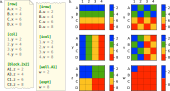
\includegraphics{figures/well_groups}
  \caption{\label{fig:well-groups}%
    \csentence{A demonstration of the most commonly-used well groups.}
    (a) A contrived layout that uses seven different well groups. Each row
    specifies a different value for the ``x'' parameter, each column a
    different value for the ``y'' parameter, etc. (b) A visualization of the
    layout in (a), as rendered by the \texttt{wellmap} command-line program. In
    each heatmap, the cells represent different wells and the colors represent
    different values of the parameter indicated on the y-axis.}
\end{figure}

\begin{figure}[h!]
  %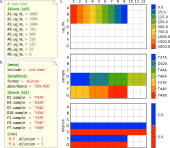
\includegraphics{figures/bradford}
  \caption{\label{fig:bradford}%
    \csentence{A real-life example of a layout used for a Bradford assay.} (a)
    A layout file describing just the concentrations of a standard curve, which
    may be relevant to many layouts. These concentrations come specifically
    from the Pierce BCA Protein Assay Kit (ThermoFisher \#23225). (b) A layout
    file describing the assay itself, including which mutants are being tested
    and what dilutions are being used.  (c) A visualization of the layout in
    (b), as rendered by the \texttt{wellmap} command-line program.}
\end{figure}

%%%%%%%%%%%%%%%%%%%%%%%%%%%%%%%%%%%
%%                               %%
%% Tables                        %%
%%                               %%
%%%%%%%%%%%%%%%%%%%%%%%%%%%%%%%%%%%

\section*{Tables}

\begin{table}[h!]

  \caption{\label{tab:pattern-syntax}
    Examples of the pattern syntax. The syntax column shows how the pattern
    would be specified in a layout file.  The meaning column shows the rows,
    columns, or wells identified by the pattern.}

  \begin{tabular}{ll}
  \toprule 
  Syntax & Meaning\\
  \midrule 
  {[}row.'A,B'{]} & A, B\\
  {[}row.'A,B,...,H'{]} & A, B, C, D, E, F, G, H\\
  {[}row.'A,C,...,G'{]} & A, C, E, G\\
  \midrule 
  {[}col.'1,2'{]} & 1, 2\\
  {[}col.'1,2,...,8'{]} & 1, 2, 3, 4, 5, 6, 7, 8\\
  {[}col.'1,3,...,7'{]} & 1, 3, 5, 7\\
  \midrule 
  {[}well.'A1,A2'{]} & A1, A2\\
  {[}well.'A1,A2,...,A6'{]} & A1, A2, A3, A4, A5, A6\\
  {[}well.'A1,C3,...,E5'{]} & A1, A3, A5, C1, C3, C5, E1, E3, E5\\
  \bottomrule
  \end{tabular}

\end{table}

\end{backmatter}
\end{document}
